%% arrowLength=10
%% linkWidth=3
%% input fy=50*node.pos
%% output fx=350
%% output fy=50*node.pos+50
%% MAX_FONT_SIZE=8
\begin{table}[H]
    \begin{center}
        \begin{tabular}{||l c c c||}
            \hline
            & 1        & 2        & 3 \\ [0.5ex]
            \hline
            velikost populacije               & 200      & 250      & 350      \\
            \hline
            največje število globokih vozlišč & 15       & 20       & 40       \\
            \hline
            največje število povezav          & 30       & 50       & 100      \\
            \hline
            največje število prečkanj         & 2        & 3        & 4        \\
            \hline
            delež mutiranih potomcev          & 10\%     & 10\%     & 10\%     \\
            \hline
            prispevek vozlišč                 & -0.00001 & -0.00001 & -0.00001 \\
            \hline
            prispevek povezav                 & -0.00001 & -0.00001 & -0.00001 \\
            \hline
            število generacij                 & 200      & 200      & 300      \\
            \hline
        \end{tabular}
    \end{center}
    \caption{Nabori inicializacijskih parametrov poganjanja na množici Car Evaluation.}
    \label{tab:param_car}
\end{table}

\subsubsection{Prvi nabor}
%%"/home/jure/CLionProjects/Neuroevolution/datasets/car/car.data" 200 15 30 2 true 0.1 100 true -0.00001 -0.00001 300 ACC
\begin{table}[H]
    \begin{center}
        \begin{tabular}{|| c | c c || c c ||}
            \hline
            \multirow{2}{*}{št. zagona} & \multicolumn{2}{c||}{točnost najboljšega agenta} & \multicolumn{2}{c||}{MCC najboljšega agenta} \\ \cline{2-5}
            & učna   & testna          & učna  & testna                  \\
            \hline
            1        & 72.0\% & 72.2\%          & 0.499 & 0.474                   \\
            \hline
            2        & 73.1\% & 71.8\%          & 0.504 & 0.461                   \\
            \hline
            3        & 75.0\% & 72.8\%          & 0.489 & 0.498                   \\
            \hline
            4        & 72.6\% & \textbf{73.2\%} & 0.482 & \textbf{0.509 (69.9\%)} \\
            \hline
            5        & 72.6\% & 73.2\%          & 0.479 & 0.428                   \\
            \hline
            $\sigma$ & 0.010  & 0.006           & 0.010 & 0.029                   \\
            \hline
        \end{tabular}
    \end{center}
    \caption{Rezultat prvega nabora parametrov.}
    \label{tab:car_result_1}
\end{table}

\begin{table}[H]
    \centering
    \begin{tabular}{||rccccc||}
        \hline
        razred       & unacceptable & acceptable & good & very good & vsota \\ \hline
        unacceptable & 357          & 6          & 0    & 0         & 363   \\ \hline
        acceptable   & 97           & 18         & 0    & 0         & 115   \\ \hline
        good         & 13           & 8          & 0    & 0         & 21    \\ \hline
        very good    & 9            & 10         & 0    & 0         & 19    \\ \hline
        vsota        & 476          & 42         & 0    & 0         & 518   \\ \hline
    \end{tabular}
    \caption{Matrika zmot najbolj točnega agenta prvega nabora. Agent lahko napove samo razreda \enquote{nesprejemljivo} in \enquote{sprejemljivo}.}
    \label{tab:car_acc_1}
\end{table}

\begin{table}[H]
    \centering
    \caption{Matrika zmot agenta z največjim MCC prvega nabora. Agent lahko napove samo razreda \enquote{nesprejemljivo} in \enquote{sprejemljivo}.}
    \begin{tabular}{||rccccc||}
        \hline
        razred       & unacceptable & acceptable & good & very good & vsota \\ \hline
        unacceptable & 260          & 103        & 0    & 0         & 363   \\ \hline
        acceptable   & 10           & 105        & 0    & 0         & 115   \\ \hline
        good         & 0            & 21         & 0    & 0         & 21    \\ \hline
        very good    & 0            & 19         & 0    & 0         & 19    \\ \hline
        vsota        & 270          & 248        & 0    & 0         & 518   \\ \hline
    \end{tabular}
    \label{tab:car_mcc_1}
\end{table}

\begin{figure}[H]
    \begin{center}
        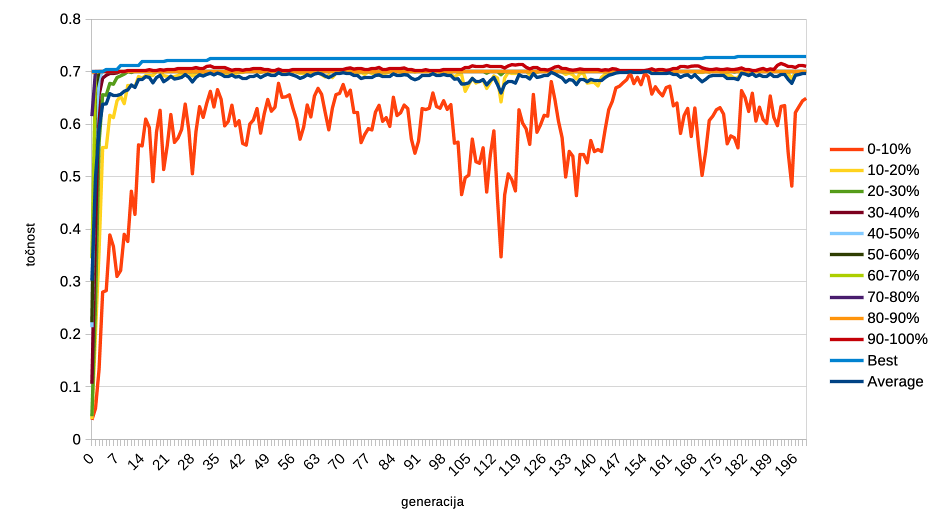
\includegraphics[width=13cm]{car/1/acc}
    \end{center}
    \caption{Graf točnosti populacije najboljšega agenta prvega nabora skozi generacije.}
    \label{fig:car_acc_1}
\end{figure}

\begin{figure}[H]
    \begin{center}
        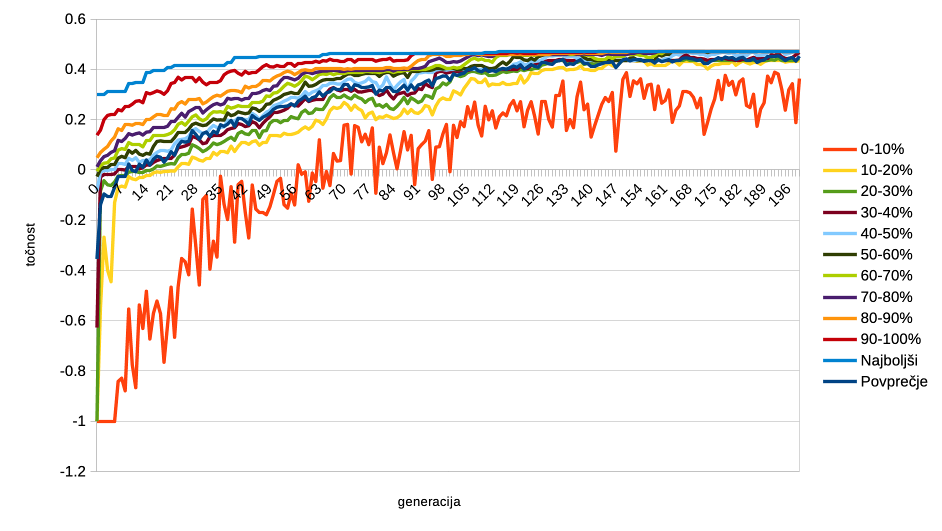
\includegraphics[width=13cm]{car/1/mcc}
    \end{center}
    \caption{Graf MCC populacije najboljšega agenta prvega nabora skozi generacije.}
    \label{fig:car_mcc_1}
\end{figure}

\begin{figure}[H]
    \begin{center}
        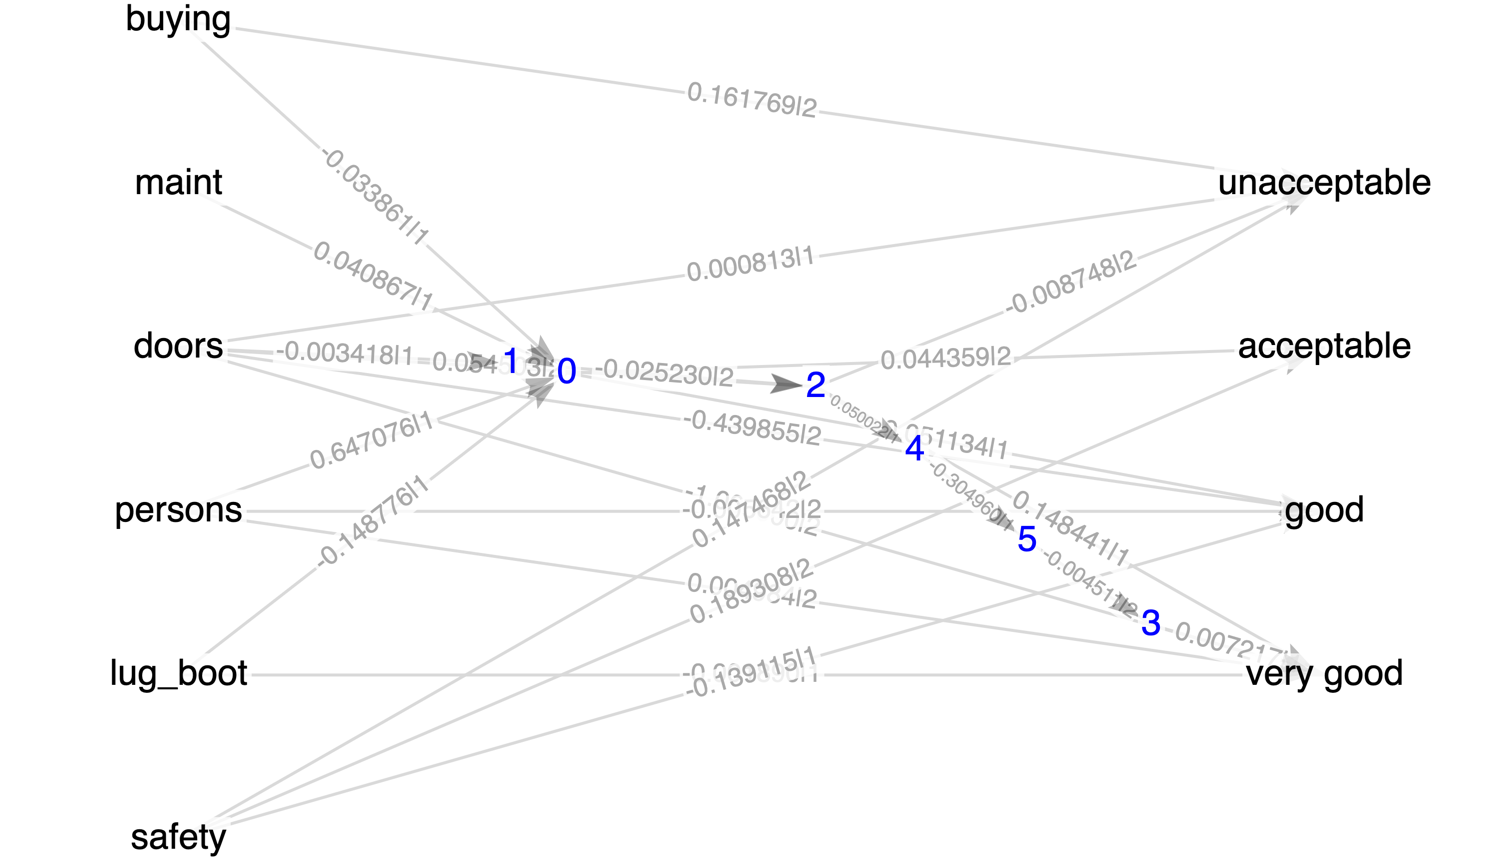
\includegraphics[width=13cm]{car/1/acc_g}
    \end{center}
    \caption{Vizualizacija najbolj točnega agenta prvega nabora. Vsebuje 6 globokih vozlišč in 25 povezav.}
    \label{fig:car_acc_1_g}
\end{figure}

\begin{figure}[H]
    \begin{center}
        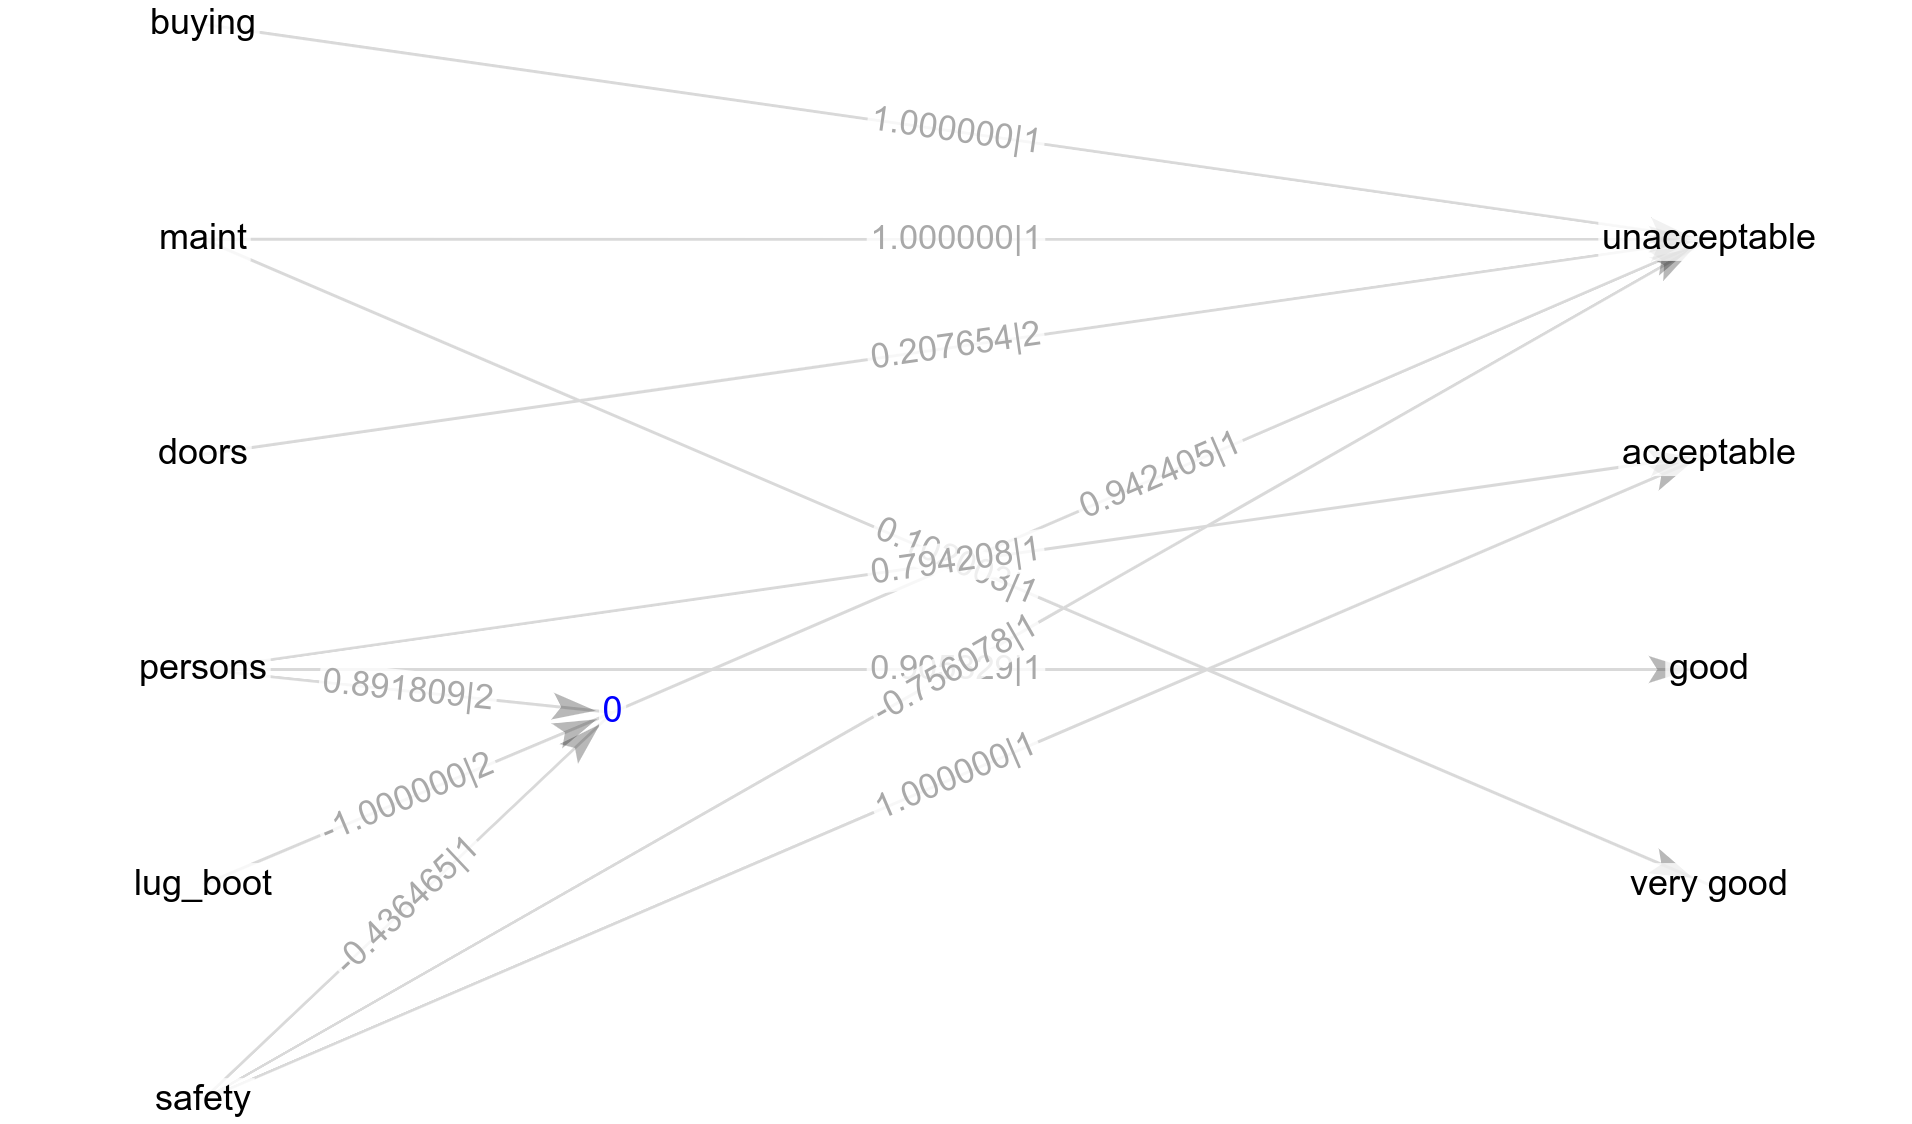
\includegraphics[width=13cm]{car/1/mcc_g}
    \end{center}
    \caption{Vizualizacija agenta z največjim MCC prvega nabora. Vsebuje 5 globokih vozlišč in 23 povezav.}
    \label{fig:car_mcc_1_g}
\end{figure}

\subsubsection{Drugi nabor}
%% 250 20 50 3 true 0.1 125 true -0.00001 -0.00001 200 ACC
\begin{table}[H]
    \caption{Rezultat drugega nabora parametrov.}
    \begin{center}
        \begin{tabular}{|| c | c c || c c ||}
            \hline
            \multirow{2}{*}{št. zagona} & \multicolumn{2}{c||}{točnost najboljšega agenta} & \multicolumn{2}{c||}{MCC najboljšega agenta} \\ \cline{2-5}
            & učna    & testna           & učna  & testna         \\
            \hline
            1        & 0.729\% & 0.716\%          & 0.505 & 0.471          \\
            \hline
            2        & 0.716\% & 0.718\%          & 0.486 & 0.507          \\
            \hline
            3        & 0.707\% & 0.701\%          & 0.475 & \textbf{0.530} \\
            \hline
            4        & 0.719\% & \textbf{0.724\%} & 0.482 & 0.513          \\
            \hline
            5        & 0.713\% & 0.695\%          & 0.501 & 0.479          \\
            \hline
            $\sigma$ & 0.007   & 0.011            & 0.011 & 0.022          \\
            \hline
        \end{tabular}
    \end{center}
    \label{tab:car_result_2}
\end{table}

\begin{table}[H]
    \centering
    \caption{Matrika zmot najbolj točnega agenta drugega nabora. Agent lahko napove samo razreda \enquote{nesprejemljivo} in \enquote{zelo dobro}.}
    \begin{tabular}{||rccccc||}
        \hline
        razred       & unacceptable & acceptable & good & very good & vsota \\ \hline
        unacceptable & 361          & 0          & 0    & 2         & 363   \\ \hline
        acceptable   & 102          & 0          & 0    & 13        & 115   \\ \hline
        good         & 15           & 0          & 0    & 6         & 21    \\ \hline
        very good    & 5            & 0          & 0    & 14        & 19    \\ \hline
        vsota        & 473          & 0          & 0    & 35        & 518   \\ \hline
    \end{tabular}
    \label{tab:car_acc_2}
\end{table}

\begin{table}[H]
    \centering
    \caption{Matrika zmot agenta z največjim MCC drugega nabora. Agent lahko napove samo razreda \enquote{nesprejemljivo} in \enquote{sprejemljivo}.}
    \begin{tabular}{||rccccc||}
        \hline
        razred       & unacceptable & acceptable & good & very good & vsota \\ \hline
        unacceptable & 276          & 87         & 0    & 0         & 363   \\ \hline
        acceptable   & 9            & 106        & 0    & 0         & 115   \\ \hline
        good         & 0            & 21         & 0    & 0         & 21    \\ \hline
        very good    & 0            & 19         & 0    & 0         & 19    \\ \hline
        vsota        & 285          & 233        & 0    & 0         & 518   \\ \hline
    \end{tabular}
    \label{tab:car_mcc_2}
\end{table}

\begin{figure}[H]
    \begin{center}
        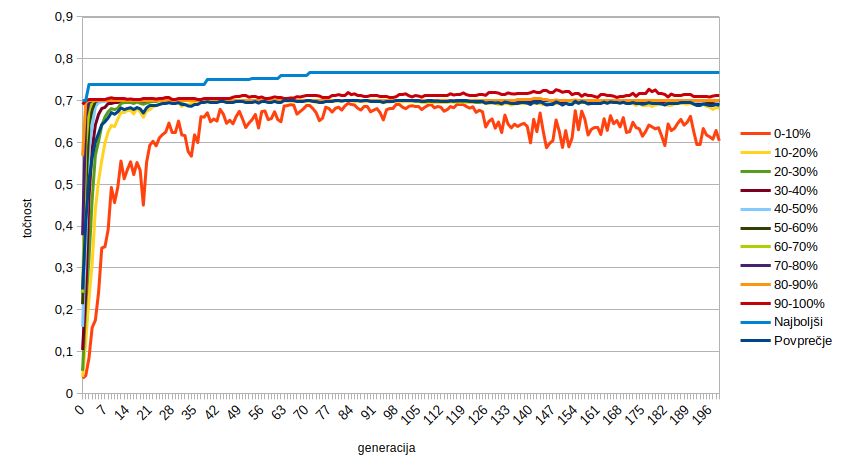
\includegraphics[width=13cm]{car/2/acc}
    \end{center}
    \caption{Graf točnosti populacije najboljšega agenta drugega nabora skozi generacije.}
    \label{fig:car_acc_2}
\end{figure}

\begin{figure}[H]
    \begin{center}
        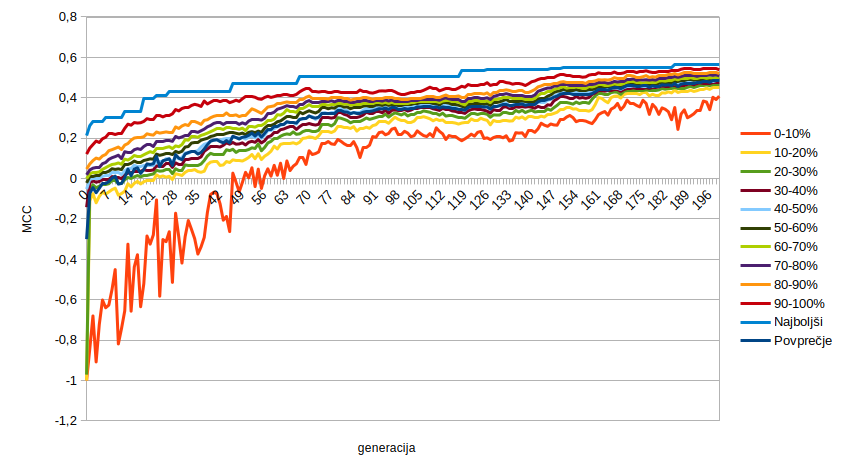
\includegraphics[width=13cm]{car/2/mcc}
    \end{center}
    \caption{Graf MCC populacije najboljšega agenta drugega nabora skozi generacije.}
    \label{fig:car_mcc_2}
\end{figure}

\begin{figure}[H]
    \begin{center}
        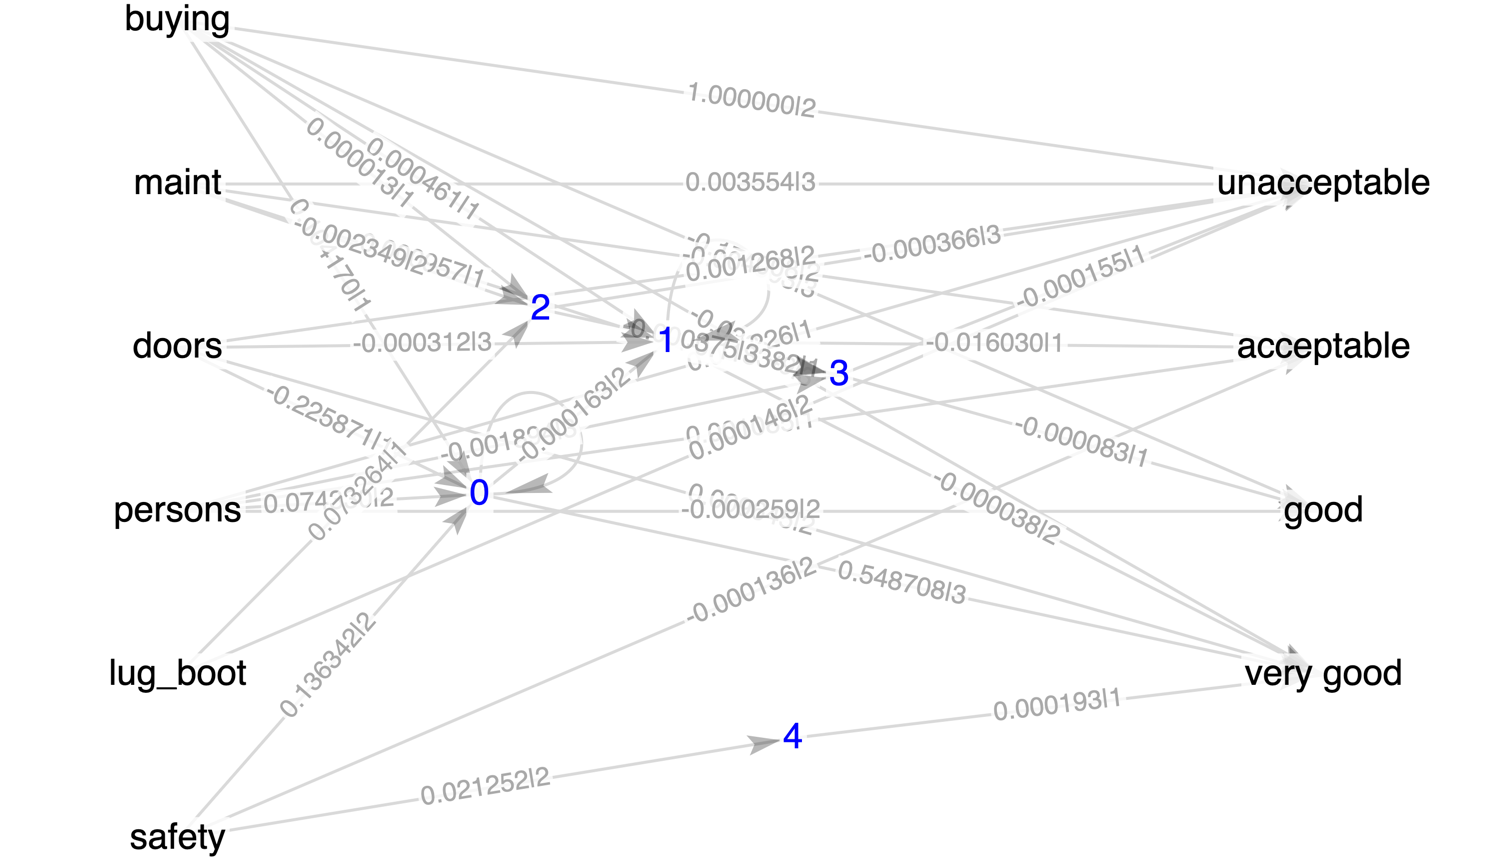
\includegraphics[width=13cm]{car/2/acc_g}
    \end{center}
    \caption{Vizualizacija najbolj točnega agenta drugega nabora. Vsebuje 5 globokih vozlišč in 36 povezav.}
    \label{fig:car_acc_2_g}
\end{figure}

\begin{figure}[H]
    \begin{center}
        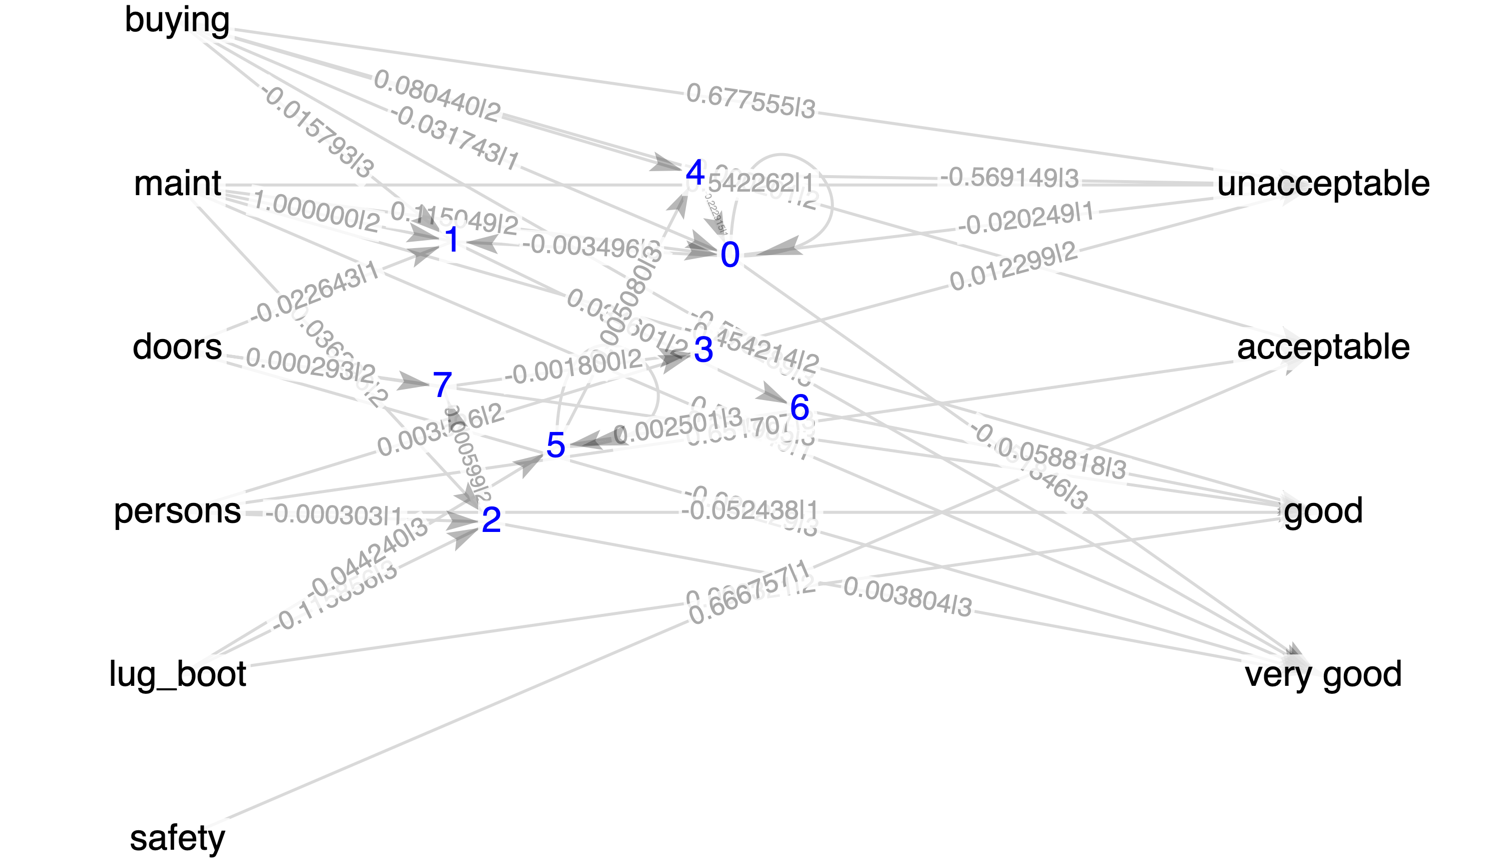
\includegraphics[width=13cm]{car/2/mcc_g}
    \end{center}
    \caption{Vizualizacija agenta z največjim MCC drugega nabora. Vsebuje 8 globokih vozlišč in 39 povezav.}
    \label{fig:car_mcc_2_g}
\end{figure}

\subsubsection{Tretji nabor}
%% 350 40 100 4 true 0.1 175 true -0.00001 -0.00001 300 ACC
\begin{table}[H]
    \caption{Rezultat tretjega nabora parametrov.}
    \begin{center}
        \begin{tabular}{|| c | c c || c c ||}
            \hline
            \multirow{2}{*}{št. zagona} & \multicolumn{2}{c||}{točnost najboljšega agenta} & \multicolumn{2}{c||}{MCC najboljšega agenta} \\ \cline{2-5}
            & učna    & testna           & učna  & testna         \\
            \hline
            1        & 0.716\% & 0.708\%          & 0.471 & 0.480          \\
            \hline
            2        & 0.719\% & 0.705\%          & 0.502 & 0.473          \\
            \hline
            3        & 0.729\% & 0.728\%          & 0.482 & \textbf{0.486} \\
            \hline
            4        & 0.740\% & 0.716\%          & 0.512 & 0.443          \\
            \hline
            5        & 0.737\% & \textbf{0.734\%} & 0.501 & 0.479          \\
            \hline
            $\sigma$ & 0.009   & 0.011            & 0.015 & 0.015          \\
            \hline
        \end{tabular}
    \end{center}
    \label{tab:car_result_3}
\end{table}

\begin{table}[H]
    \centering
    \caption{Matrika zmot najbolj točnega agenta tretjega nabora. Agent lahko napove samo razreda \enquote{nesprejemljivo} in \enquote{sprejemljivo}.}
    \begin{tabular}{||rccccc||}
        \hline
        razred       & unacceptable & acceptable & good & very good & vsota \\ \hline
        unacceptable & 306          & 57         & 0    & 0         & 363   \\ \hline
        acceptable   & 41           & 74         & 0    & 0         & 115   \\ \hline
        good         & 0            & 21         & 0    & 0         & 21    \\ \hline
        very good    & 0            & 19         & 0    & 0         & 19    \\ \hline
        vsota        & 347          & 171        & 0    & 0         & 518   \\ \hline
    \end{tabular}
    \label{tab:car_acc_3}
\end{table}

\begin{table}[H]
    \centering
    \caption{Matrika zmot agenta z največjim MCC tretjega nabora. Agent lahko pravilno napove samo razreda \enquote{nesprejemljivo} in \enquote{sprejemljivo}.}
    \begin{tabular}{||rccccc||}
        \hline
        razred       & unacceptable & acceptable & good & very good & vsota \\ \hline
        unacceptable & 267          & 88         & 0    & 8         & 363   \\ \hline
        acceptable   & 13            & 102        & 0    & 0         & 115   \\ \hline
        good         & 0            & 21         & 0    & 0         & 21    \\ \hline
        very good    & 0            & 19         & 0    & 0         & 19    \\ \hline
        vsota        & 280          & 230        & 0    & 8         & 518   \\ \hline
    \end{tabular}
    \label{tab:car_mcc_3}
\end{table}

\begin{figure}[H]
    \begin{center}
        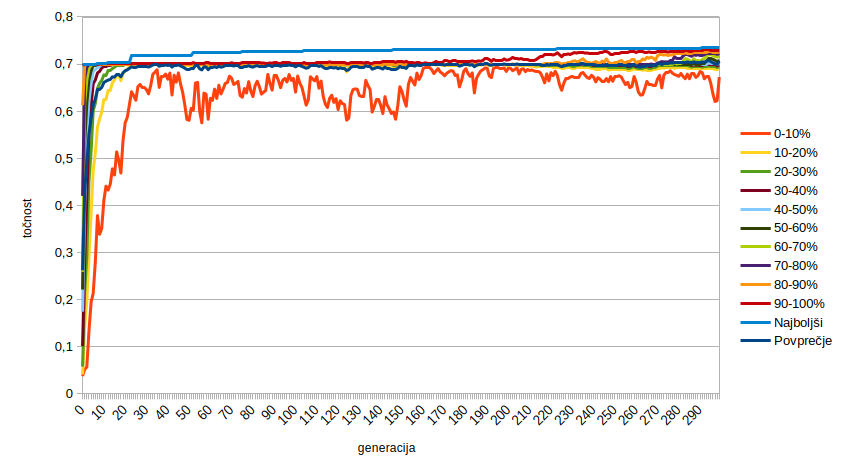
\includegraphics[width=13cm]{car/3/acc}
    \end{center}
    \caption{Graf točnosti populacije najboljšega agenta tretjega nabora skozi generacije.}
    \label{fig:car_acc_3}
\end{figure}

\begin{figure}[H]
    \begin{center}
        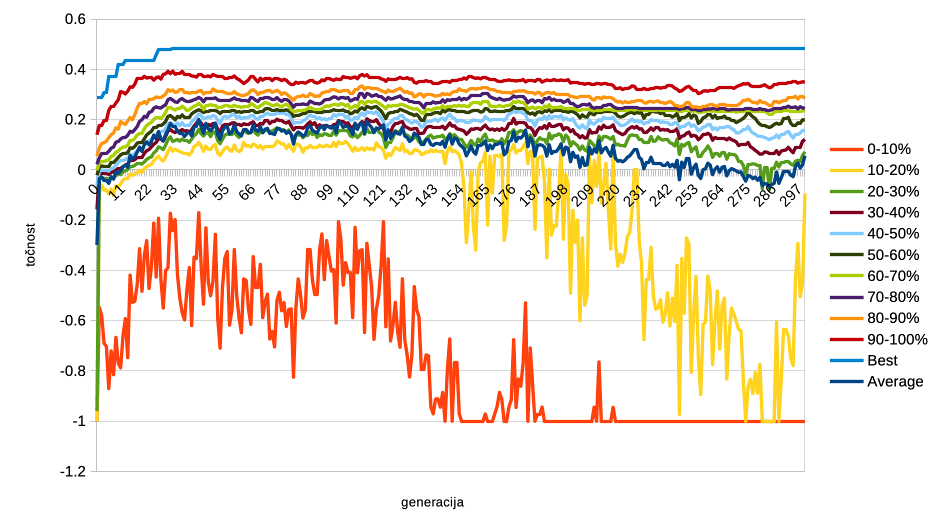
\includegraphics[width=13cm]{car/3/mcc}
    \end{center}
    \caption{Graf MCC populacije najboljšega agenta tretjega nabora skozi generacije.}
    \label{fig:car_mcc_3}
\end{figure}

\begin{figure}[H]
    \begin{center}
        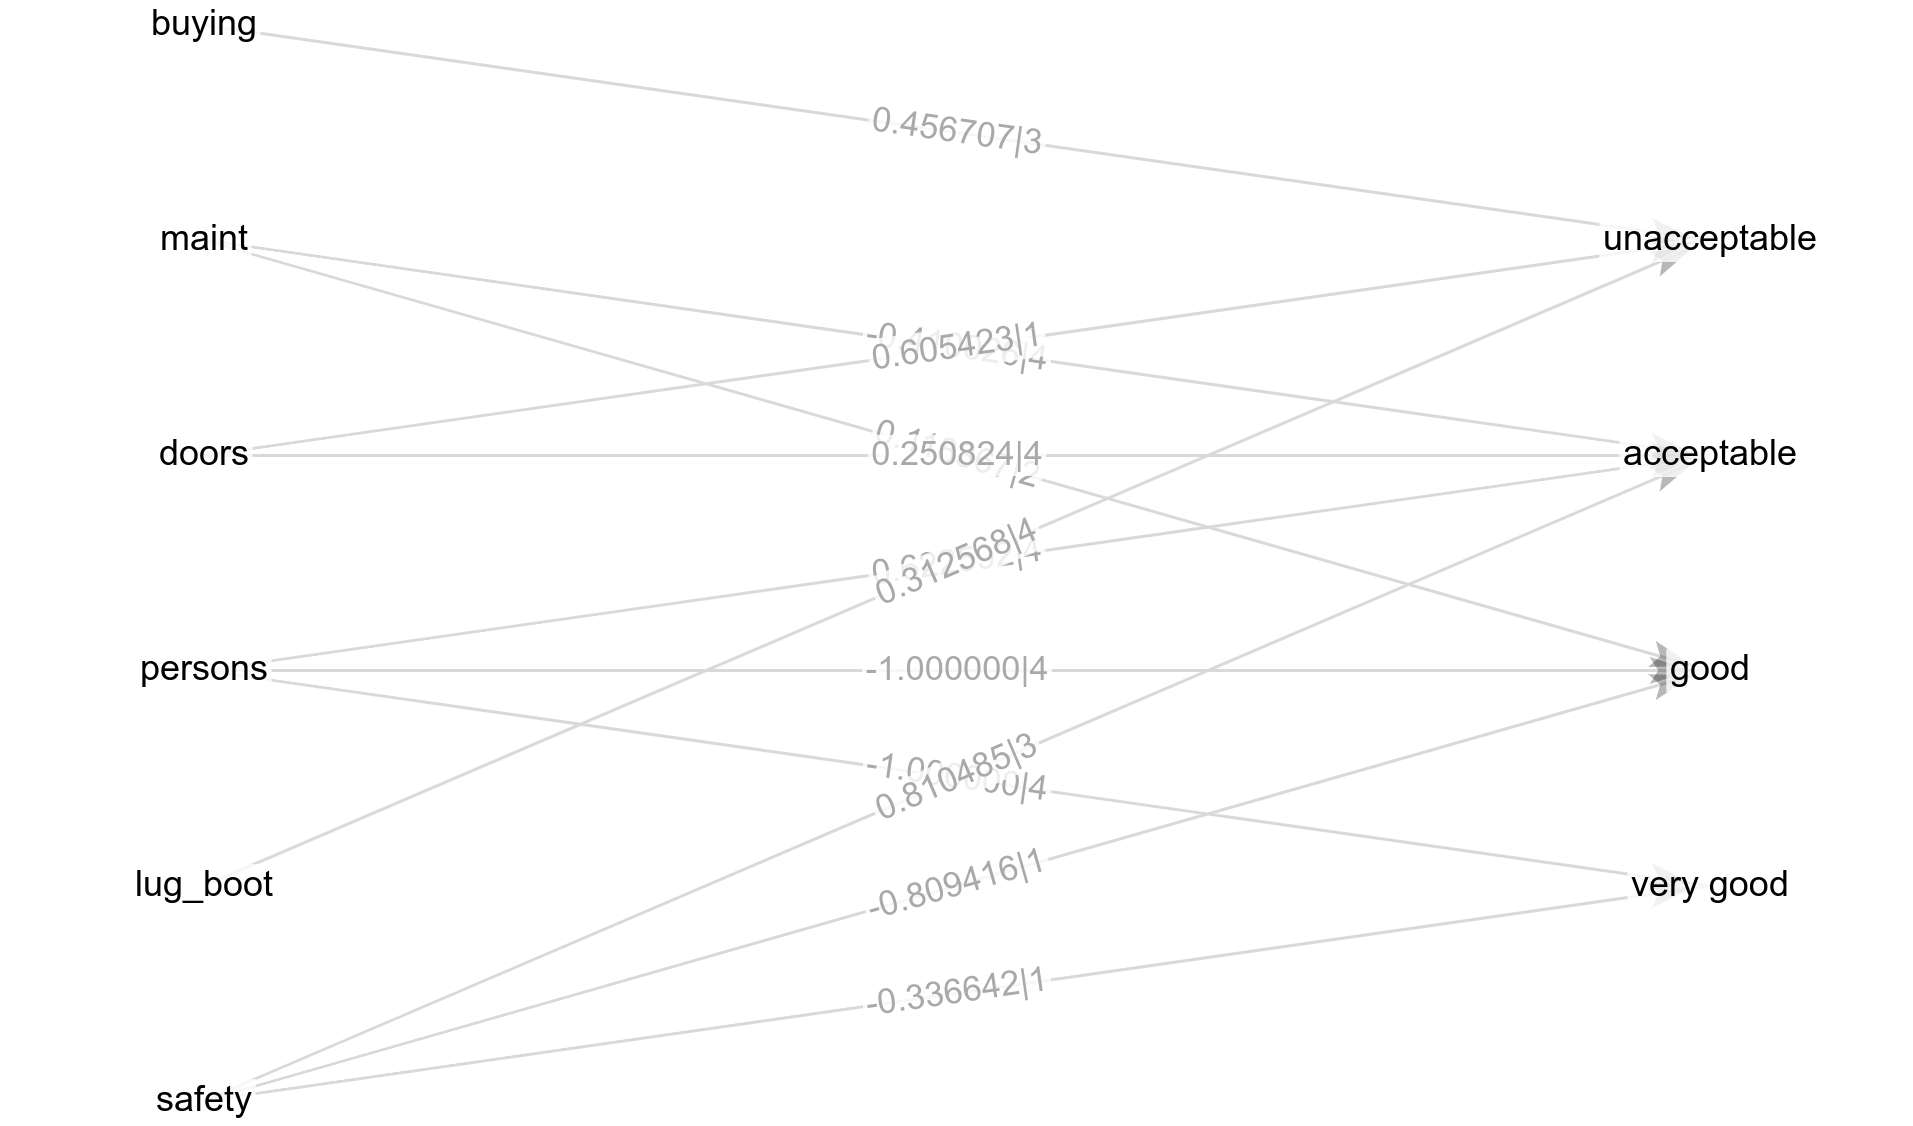
\includegraphics[width=13cm]{car/3/acc_g}
    \end{center}
    \caption{Vizualizacija najbolj točnega agenta tretjega nabora. Vsebuje 15 globokih vozlišč in 64 povezav.}
    \label{fig:car_acc_3_g}
\end{figure}

\begin{figure}[H]
    \begin{center}
        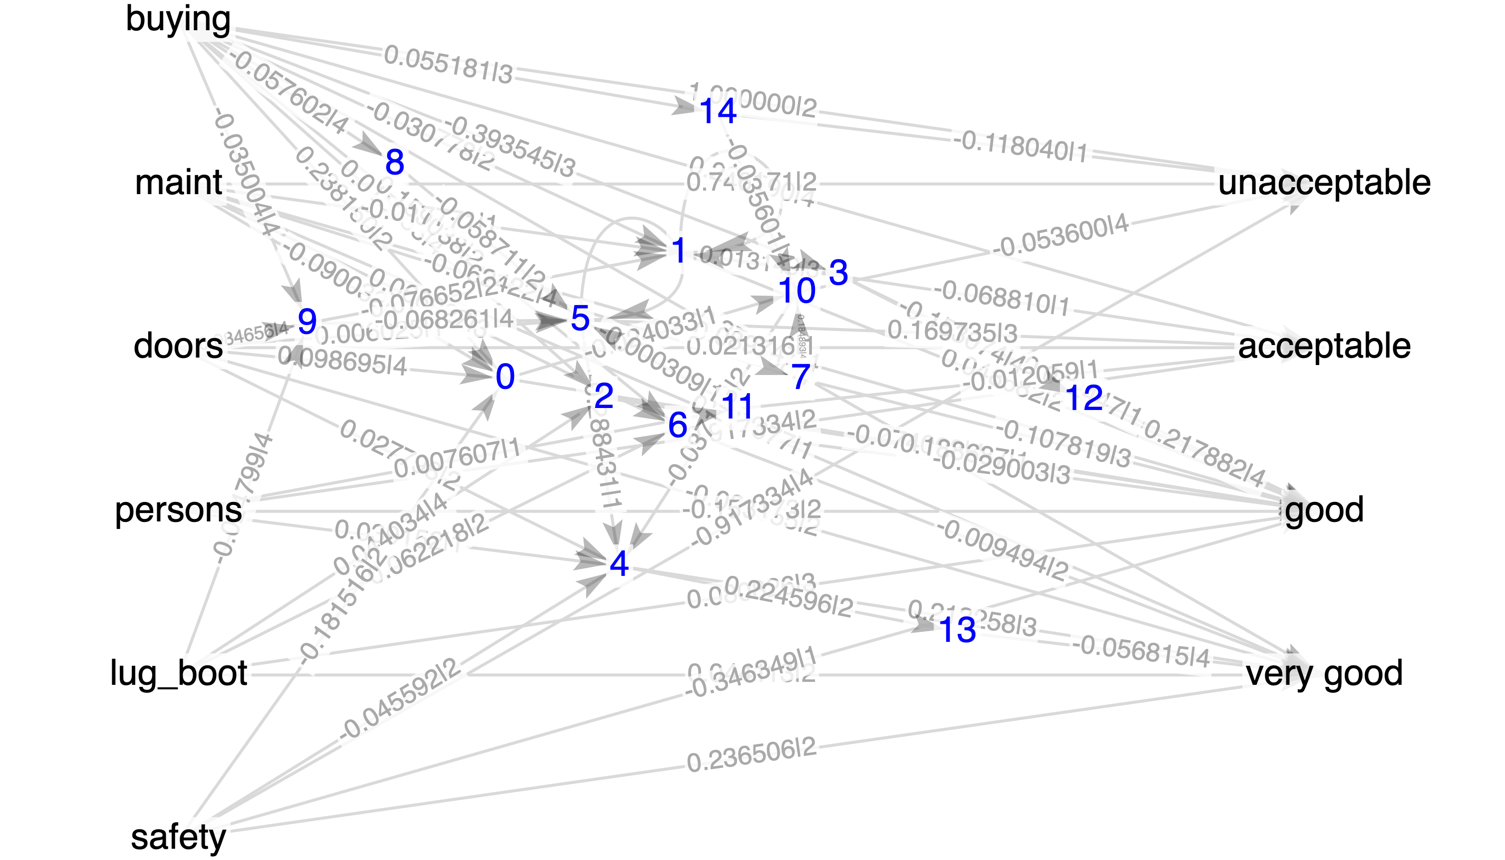
\includegraphics[width=13cm]{car/3/mcc_g}
    \end{center}
    \caption{Vizualizacija agenta z največjim MCC drugega nabora. Vsebuje 15 globokih vozlišč in 67 povezav.}
    \label{fig:car_mcc_3_g}
\end{figure}